\documentclass{article}
\setlength{\parskip}{5pt} % esp. entre parrafos
\setlength{\parindent}{0pt} % esp. al inicio de un parrafo
\usepackage{amsmath} % mates
\usepackage[sort&compress,numbers]{natbib} % referencias
\usepackage{url} % que las URLs se vean lindos
\usepackage[top=25mm,left=20mm,right=20mm,bottom=25mm]{geometry} % margenes
\usepackage{hyperref} % ligas de URLs
\usepackage{graphicx} % poner figuras
\usepackage[spanish]{babel} % otros idiomas
\usepackage[utf8]{inputenc} % alparecer son los acentos
\author{I E G} % author
\title{Práctica 1} % titulo
\date{\today}

\begin{document} % inicia contenido

\maketitle % cabecera

\begin{abstract} % resumen
En esta práctica se realiza la simulación del movimiento Browniano de una partícula en el cual se analiza sistemáticamente la relación de la distancia Manhattan de la partícula desde su punto de origen hasta su punto final y las dimensiones del espacio.
\end{abstract}

\section{Introducci\'{o}n}\label{intro} % seccion y etiqueta
 
Para esta práctica se realiza modificaciones al código fuente \cite{elis} donde se agrega filtros de datos y parámetros del código para tener una gráfica estética.




\begin{figure} % figura
    \centering
    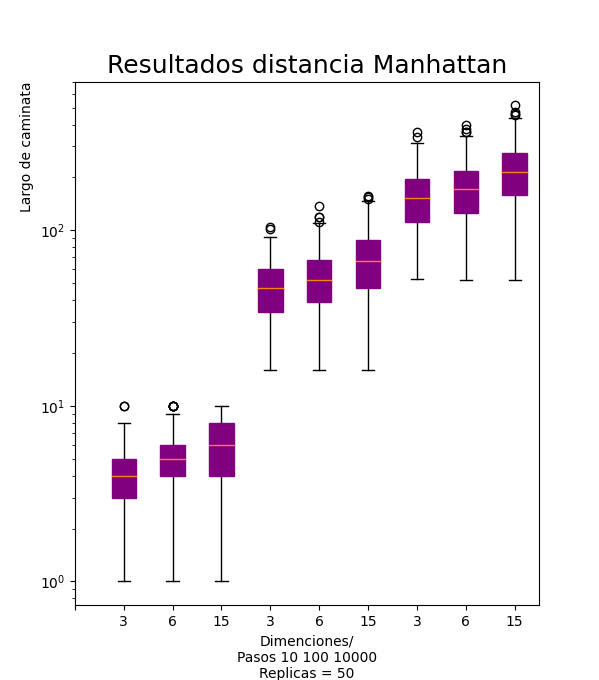
\includegraphics[width=90mm]{figuraprac1.png} % archivo
    \caption{resultados de la simulación}
    \label{grafica}
\end{figure}

\section{Desarrollo}

Se usa el código de \cite{elis} para la generación de datos, esta información se almacena en tres DataFrame que son filtrados para graficar de forma ordenada los datos en una gráfica caja bigote, la sección de filtrado funciona almacenando los datos de las diferentes corridas en pasos de 10, 100 y 10000.

 
\begin{lstlisting}[language = python]

datos = pd.DataFrame(data, columns = ['Dim', 'Dur', 'Rep', 'Dist'])


g1 = datos[datos['Dur'] == 10]

g2 = datos[datos['Dur'] == 1000]

g3 = datos[datos['Dur'] == 10000]
\end{lstlisting}


Cuando los datos están filtrados se grafica con el paquete de Matplotlib.

\begin{lstlisting}[language = python]
plt.boxplot([g1['Dist'], g16['Dist'], g115['Dist'], g2['Dist'], g26['Dist'], g215['Dist'], g3['Dist'], g36['Dist'], g315['Dist']], patch_artist=True, boxprops=dict(facecolor=c, color=c))
\end{lstlisting}

Los parámetros especiales para la estética de la gráfica se toman de \url{https://matplotlib.org/stable/contents.html} donde se encuentra la documentación oficial de Matplotlib.

\section{Conclusiones}

En conclusión el aumento de las dimensiones de Figura \ref{grafica} incrementa la media de la posición final de la partícula así que se puede suponer que en mayores dimensiones en la que se encuentra una partícula mayor seria su energía pues puede moverse a mayor distancia que a menores dimensiones.
\bibliography{simu}
\bibliographystyle{plainnat}

\end{document}